%----------------------------------------------------------------------------
\chapter{Számítógépes elemzés}
%----------------------------------------------------------------------------
Ebben a fejezetben bemutatom az előző fejezetben elviekben ismertetett modelleket példákon és valós adatokon keresztül. A szoftver segítségünkre lesz abban, hogy megoldjuk a felmerülő differenciálegyenleteket és egyenletrendszereket, végül az eredményeket grafikus felületen is megtekinthetjük.

\begin{figure}[!h]
	\centering
	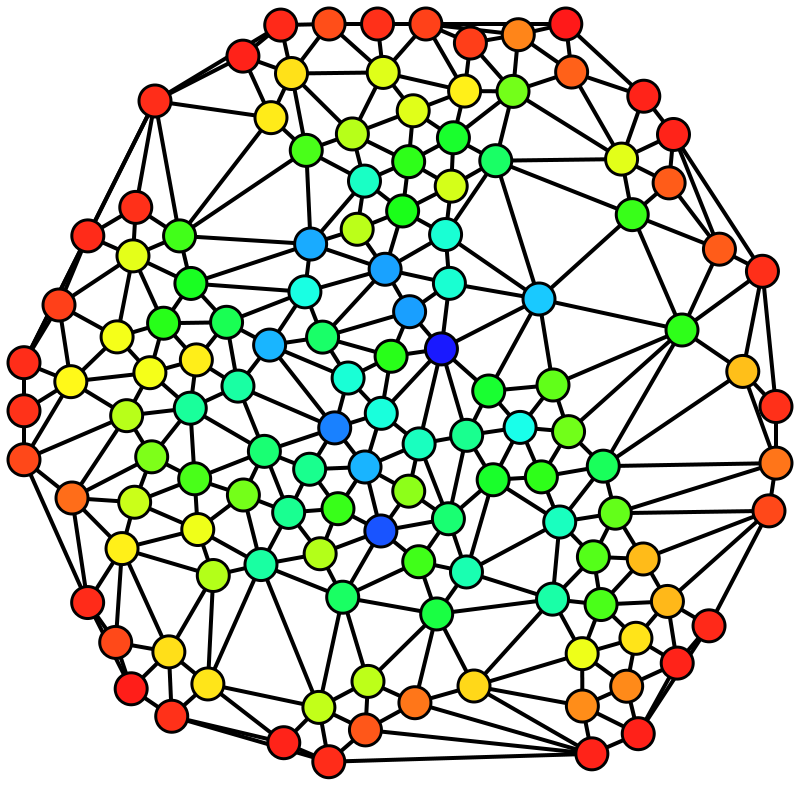
\includegraphics[scale=0.2]{images/graf1}
	\caption{Gr\'af}
\end{figure}


\begin{figure}[!h]
	\centering
	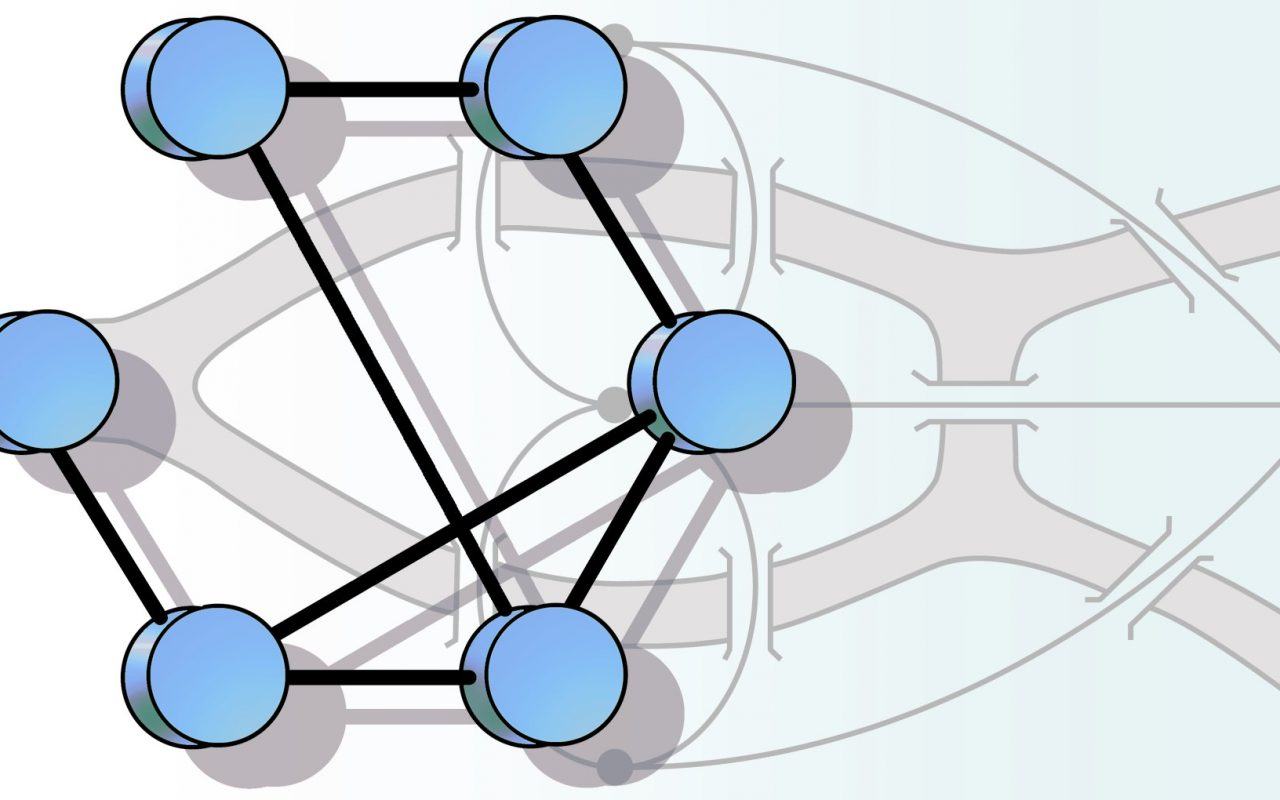
\includegraphics[scale=0.2]{images/graf2}
	\caption{Gr\'af 2}
\end{figure}


\begin{figure}[!h]
	\centering
	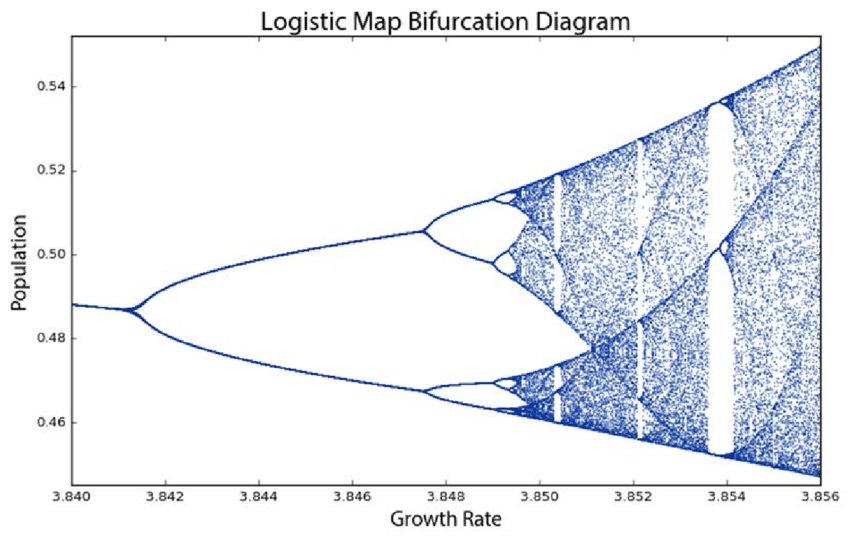
\includegraphics[scale=0.3]{images/kep2}
	\caption{Bifurk\'aci\'os diagram}
\end{figure}



\begin{figure}[!h]
	\centering
	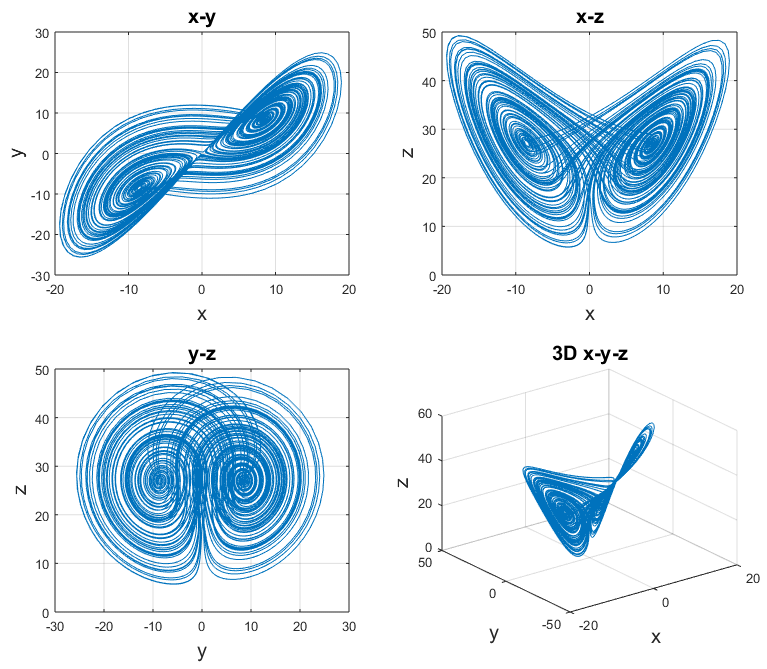
\includegraphics[scale=0.4]{images/kep33}
	\caption{Lorentz attraktor}
\end{figure}